\documentclass[11pt,spanish]{article} % Tipo y tamaño de letra del documento.


\usepackage[utf8]{inputenc}
\usepackage{subfiles}
\usepackage{biblatex}
\addbibresource{references.bib}
\usepackage{multicol}
\usepackage{amsfonts}
\usepackage{blindtext}
\usepackage{mathrsfs}
\usepackage{amsmath}
\usepackage{siunitx}
\usepackage{centernot}
\usepackage[shortlabels]{enumitem}
\usepackage{subfig}
\usepackage{datetime}
\usepackage{listingsutf8}
\usepackage[spanish]{babel}
\usepackage{tikz}
\usepackage{hyperref}
\usepackage[vlined,ruled,linesnumbered]{algorithm2e}
\usepackage{listings}
\usepackage{float}
\usepackage{url}
\usepackage{csquotes}
\usepackage{fourier} %font
\usepackage[top=2cm, bottom=2cm, left=2.5cm, right=2.5cm]{geometry}
\usepackage{pgfplots}
\usepackage{fancyhdr}
\usepackage{mdframed}
\usepackage{tikzducks}
\usepackage[nameinlink]{cleveref}
\usepackage{epigraph} 

\pgfplotsset{compat=1.18}

\usetikzlibrary{shapes.arrows, shapes.geometric, arrows.meta,angles,quotes,positioning,arrows,fit,quotes,calc}
\tikzset{>=latex} 

\setlength\algomargin{1em} 
\SetFuncSty{sc} 
\SetCommentSty{em} 


\Crefname{figure}{Fig.}{Figs.}
\newcommand\crefrangeconjunction{--}
\Crefname{table}{Tabla}{Tablas}
\Crefname{subsubsection}{Subsubsec.}{Subsubsections}
\Crefname{subsection}{Subsec.}{Subsections}
\Crefname{section}{Sec.}{Sections}
\Crefname{equation}{eq.}{eqs.}
\crefname{thm}{Theorem}{theorems}
\Crefname{thm}{Theorem}{Theorems} 

\definecolor{algoco}{rgb}{0,0.4,1}

\hypersetup{
  colorlinks=true,
  linkcolor=algoco,
  citecolor=blue,
  urlcolor=blue,
}

\lstset{
extendedchars=true
inputencoding=utf8/latin1,
basicstyle=\footnotesize\sffamily\color{black},
commentstyle=\slshape \color{gray},
numbers=left,
numbersep=10pt,
numberstyle=\tiny\color{red!80!black},
keywordstyle=\color{red!80!magenta},
showspaces=false,
showstringspaces=false,
stringstyle=\color{cyan!80!black},
tabsize=2,
literate={á}{{\'a}}1 {é}{{\'e}}1 {í}{{\'i}}1 {ó}{{\'o}}1 {ú}{{\'u}}1,
frame = single, 
numbers = none,
float, floatplacement = ht, captionpos = b,
xleftmargin = 2em, xrightmargin = 2em, 
}

\newcommand{\ub}[1]{\underbrace{#1}}
\newcommand\tcm{\textcolor{magenta}}
\newcommand\tca{\textcolor{algoco}}

\setlength\epigraphwidth{.7\textwidth} 

\newcommand{\tnum}{2 y 3} % reemplace 2 por el número de la tarea
\newcommand{\sem}{2024-2} % reemplace 2024-2 por el semestre correspondiente
\newcommand{\campus}{San Joaquin \\ Santiago} % reemplace Casa Central por el campus correspondiente
\newcommand{\rolusm}{202160584-3} % reemplace 2025073100-1 por su rol
\newcommand{\namestudent}{Franco Sepúlveda} % reemplace Al Goritmo Pérez por su nombre

\headheight=14pt
\linespread{1.3}
\author{\namestudent}
\pagestyle{fancy}
\fancyhf{}%
\fancyfoot[R]{ \namestudent \\ \rolusm}
\fancyfoot[L]{Campus \campus} 
\fancyfoot[C]{\thepage}
\rhead{2024-2}
\lhead{INF-221}
\renewcommand{\headrulewidth}{0.4pt}
\renewcommand{\footrulewidth}{0.4pt}
\newbool{programs}
\boolfalse{programs}
\chead{REPORTE TAREA \tnum~}



\title{
  \huge
  \textbf{REPORTE TAREA \tnum~ \\ ALGORITMOS Y COMPLEJIDAD} \\[1ex]
  \emph{\textquote{Explorando la Distancia entre Cadenas, una Operación a la Vez}}
  }

  
\date{
  \small
  \today\\
  \currenttime
}




\begin{document}
\maketitle
\thispagestyle{fancy} 
\vspace{-1.0\baselineskip}




\begin{abstract}
  \textit{ 
    Esta tarea aborda el problema de calcular la distancia mínima de edición entre dos cadenas de texto, utilizando algoritmos de Programación Dinámica y Fuerza Bruta. El objetivo es calcular esta distancia mediante operaciones de inserción, eliminación, sustitución y transposición, cada una con un costo asociado.
El informe incluye la contextualización del problema y su relevancia, presenta los algoritmos junto con ejemplos de su aplicación y análisis de su complejidad(temporal y espacial),explica la estructura y funcionamiento de los programas desarrollados, mide los tiempos de ejecución sometiendo los algoritmos a cadenas de distintas características y finalmente interpreta los resultados.

La importancia de este problema radica en mejorar la eficiencia en tareas como la corrección ortográfica, el análisis de texto y la biología computacional.




  }
     
\end{abstract}

\setcounter{tocdepth}{1}
\tableofcontents


\newpage
\section{Introducción}
La distancia mínima entre dos cadenas surge como solución a el problema de corrección de errores en códigos de información, en particular, a la necesidad de medir la diferencia entre dos cadenas de texto o secuencias, determinando el numero mínimo de transformaciones 
necesarias para convertir una cadena en otra. 
Esta solución, conocida como "La distancia de Levenshtein" pertenece al campo de Análisis y Diseño de algoritmos en Ciencias de la Computación, un área crucial en la resolución de problemas complejos con impacto significativo tanto en aplicaciones prácticas como en la investigación académica.\\

Tal vez muchas personas, yo incluido, no tenian en cuenta la relevancia  que puede tener la solucion a problemas de correccion de errores, pero esto se puede ver reflejado en la aplicabilidad en ámbitos de la vida real que tiene este problema, tales como:

-Correccion ortográfica: Consiste en sugerir la palabra correcta cuando un usuario 
comete errores tipográficos.

-Motores de búsqueda: Ayuda a mejorar los resultados de búsqueda cuando hay errores
tipográficos o variaciones en las palabras.

-Biología computacional: Aplicado en secuencias de ADN, ARN o proteínas.
En este caso se mide la "distancia" entre secuencias genéticas para detectar mutaciones
o comparar diferentes organismos.

-Comparación de textos para análisis de plagio: Compara textos y detecta
similitudes o plagio entre documentos.

-Machine learning y natural languaje processing: La distancia se usa como una métrica
de similitud para entrenar modelos de aprendizaje automático en el campo de procesamiento
de lenguaje natural(NLP). Útil en tareas como traducción automática,
reconocimiento de entidades nombradas,etc.\\

En este trabajo se aplicará la distancia de Levenshtein pero con ciertas modificaciones,
agregando la operación de transposición y variando los costos de las operaciones.
¿Como afecta la inclusión de transposición y costos variables? Este informa busca 
responder a esta cuestión mediante el análisis de dos enfoques: un algoritmo basado en
programación dinámica y otro en fuerza bruta, aplicados a este problema extendido.

Se compararan ambas implementaciones en términos de estructura, tiempos de ejecución y uso de memoria al procesar cadenas con distintas características.
Esta comparación entre paradigmas distintos permite comprender la relación entre la complejidad teorica y los resultados experimentales, parte esencial para un curso de pregrado. 



\newpage
\section{Diseño y Análisis de Algoritmos} 
\input{sections/design_analysis}

\subsection{Fuerza Bruta}

\subsubsection{Descripción solución diseñada}
Para implementar la distancia mínima entre dos cadenas utilizando fuerza bruta se pasan como parametros la cadena 1(s1), la cadena 2(s2), n(tamaño s1) y m(tamaño s2), en este algoritmo ambas cadenas se recorreran recursivamente desde sus caracteres finales hasta sus caracteres iniciales. \\
Primero se identificaron 3 casos base, cuando la cadena 1 es vacía, en este caso el costo total corresponderá al costo de insertar todas las letras de la cadena 2.
Cuando la cadena 2 es vacía, aquí el costo total corresponderá al costo de eliminar todas las letras de la cadena 1.
Y el ultimo caso es cuando las dos letras apuntadas en ambas cadenas son iguales, en este caso se procede a llamar recursivamente a la función para acceder a la siguiente letra de la cadena 1 y de la cadena 2.\\
Luego de los casos bases, se procede a llamar recursivamente a la función con el fin de calcular los costo de insertar, eliminar, sustituir y transponer, quedandose con el minimo entre estos. 
Al ser de fuerza bruta, este algoritmo calculará todos los costos de todas las combinaciones posibles, de esta forma se irá quedando cada vez con el costo menor entre los 4 calculados. Y así seguirá hasta quedarse finalmente con el costo mínimo de todas las recursiones hechas.
\subsubsection{Análisis temporal y espacial}
n: Tamaño cadena 1.
m: Tamaño cadena 2.

Análisis temporal: El peor caso ocurre cuando los caracteres del mismo indice entre las dos cadenas no son iguales y cuando se cumplen las condiciones para transponer, al cumplirse esto, se hacen siempre las 4 recursiones. Esto genera un crecimiento exponencial en el numero total de operaciones ya que cada subproblema genera hasta 4 nuevos subproblemas, formando un arbol de recursión aproximadamente de altura min(n,m). Por lo tanto, la complejidad en el peor caso es:
\[O(4^{max(n,m)})\]
Analisis espacial: El programa al no usar estructuras de datos adicionales, el análisis espacial solo se hace sobre el stack, en el peor caso, el algoritmo realiza como máximo n + m recursiones, ya que en cada llamada recursiva al menos uno de los indices n o m disminuye. Esto asegura que la profundidad máxima de la pila estará acotada por la suma de los tamaños de las cadenas(n y m). La complejidad espacial queda:
\[O(n+m)\]
\subsubsection{Algoritmo utilizando fuerza bruta}
\begin{algorithm}[H]
    \SetKwProg{myproc}{Procedure}{}{}
    \SetKwFunction{distanciaFB}{distanciaFB}  % Cambia 'AlgorithmName' por el nombre del enfoque elegido
    
    \DontPrintSemicolon
    \footnotesize

    % Definición del algoritmo principal
    \myproc{\distanciaFB{s1, s2, n, m}}{
    \uIf{n = 0}{
    	$costo \leftarrow 0$\;
    	\For{$i \leftarrow 0$ \KwTo $m$}{
    		$costo \leftarrow costo + costo\_ins(s2[i])$\;
    	}
        \Return $costo$;  
    }
    \uIf{m = 0}{
    	$costo \leftarrow 0$\;
    	\For{$i \leftarrow 0$ \KwTo $n$}{
    		$costo \leftarrow costo + costo\_del(s1[i])$\;
    	}
    	\Return $costo$; 
    }
    
    
    \uIf{s1[n-1] = s2[m-1]}{
    	\Return \distanciaFB{s1,s2,n-1,m-1}; 
    }
    
    
    $costo\_insertar = \distanciaFB(s1,s2,n,m-1) + costo\_ins(s2[m-1])$;
    
    $costo\_delete = \distanciaFB(s1,s2,n-1,m) + costo\_del(s1[n-1])$;
    
    $costo\_sustituir  = \distanciaFB(s1,s2,n-1,m-1) + costo\_sub(s1[n-1],s2[m-1])$;
    
    $costo\_transponer = INT\_MAX$;
    
    \uIf{($s1[n-1] = s2[m-2]$ \textbf{and} $s1[n-2] = s2[m-1]$ \textbf{and} $n > 1$ \textbf{and} $m > 1$)}{
    	$costo\_transponer \gets distanciaFB(s1, s2, n-2, m-2) + costo\_trans(S1[n-1], S1[n-2])$\;
    }
    
    
    \Return $\min(costo\_insertar,costo\_delete,costo\_sustituir,costo\_transponer)$;
    
    }
    \caption{Algoritmo de fuerza bruta para encontrar la distancia.}
    \label{alg:mi_algoritmo_1}
\end{algorithm}

\subsubsection{Ejemplo paso a paso}
Dadas las cadenas: s1 = $"$ab$"$,  s2 = $"$ba$"$. Si los costos de las operaciones son:
Inserción : 1, Eliminación: 1, Sustitución : 1, Transposición : 1


\subsection*{Llamada inicial}
La llamada inicial es: distanciaFB($"$ab$"$, $"$ba$"$, 2, 2).
Evaluación paso a paso

1. Caso general: \( s1[1] \neq s2[1] \).\\
   Evaluamos los costos de cada operación: Costo insertar: distanciaFB($"$ab$"$, $"$ba$"$, 2, 1) + 1, Costo eliminar: distanciaFB($"$ab$"$, $"$ba$"$, 1, 2) + 1, Costo sustituir: distanciaFB($"$ab$"$, $"$ba$"$, 1, 1) + 1, Costo transponer: distanciaFB($"$ab$"$, $"$ba$"$, 0, 0) + 1 (condición cumplida).

2. Subproblema: distanciaFB($"$ab$"$, $"$ba$"$, 1, 1): \( s1[0] \neq s2[0] \), evaluamos los costos: Costo insertar: distanciaFB($"$ab$"$, $"$ba$"$, 1, 0) + 1 = 2, Costo eliminar: distanciaFB($"$ab$"$, $"$ba$"$, 0, 1) + 1 = 2, Costo sustituir: distanciaFB($"$ab$"$, $"$ba$"$, 0, 0) + 1 = 1.
  El mínimo es \( 1 \), correspondiente a la sustitución.\\

3. Subproblema  distanciaFB($"$ab$"$, $"$ba$"$, 1, 2):
   - Evaluamos los costos:
   Costo insertar: distanciaFB($"$ab$"$, $"$ba$"$, 1, 1) + 1 = 2, 
   Costo eliminar: distanciaFB($"$ab$"$, $"$ba$"$, 0, 2) + 1 = 3.
   
   El mínimo es \( 2 \).\\

4. Subproblema distanciaFB($"$ab$"$, $"$ba$"$, 2, 1):**
   - Evaluamos los costos:
   
   Costo eliminar: distanciaFB($"$ab$"$, $"$ba$"$, 1, 1) + 1 = 2.
   
   El mínimo es \( 2 \).\\

5. Resolviendo distanciaFB($"$ab$"$, $"$ba$"$, 2, 2):

   Costo transponer: distanciaFB($"$ab$"$, $"$ba$"$, 0, 0) + 1 = 1.

   El mínimo global es \( 1 \), correspondiente a la transposición.

\subsection*{Resultado}
Finalmente el costo mínimo para transformar \( s1 \) en \( s2 \) es:
\[
\text{distanciaFB($"$ab$"$, $"$ba$"$, 2, 2)} = 1.
\]

\subsubsection{Impacto de incluir operación de transposición y costos variables en la complejidad}
La inclusión de la operación de transposicion genera que se haga una recusión más, lo que causa que la complejidad original \(O(3^{min(n,m)})\) pase a \(O(4^{min(n,m)})\), esto provoca un crecimiento exponencial aún más rapido. 
Lo que puede provocar que el algoritmo sea impráctico para cadenas de mayor tamaño.
La complejidad espacial sigue siendo de \(O(n+m)\) ya que cada llamada recursiva sigue disminuyendo al menos uno de los indices n o m.

Por otro lado, los costos variables aportan flexibilidad para modelar problemas más realistas, pero no afectan directamente la estructura del arbol de recursión. Sin embargo, puede incrementar la carga computacional en cada nivel debido a que para cada costo debe acceder a las tablas de costos, y aunque esta operación sea de O(1), la acumulación de estos acceso en la ejecución completa del algoritmo puede incrementar el tiempo de cálculo.

En conclusión, aumenta la complejidad temporal de \(O(3^{max(n,m)})\)  a \(O(4^{max(n,m)})\) y la complejidad espacial se mantiene \(O(n+m)\).
\subsection{Programación Dinámica}
\subsubsection{Descripción de la solución recursiva}
Para implementar la solución mediante programación dinámica se utilizó el enfoque bottom up. Primero se crea una tabla de tamaño $(n+1) \times (m+1)$, que representa los subproblemas para medir la distancia entre prefijos de las cadenas s1 y s2. Luego esta se inicializa en la función \texttt{inicializarMatriz}. Inicialización: 

-tabla[0][0] = 0, que corresponde al caso en que ambas cadenas están vacías.

-Primera fila(n=0): Representa cuando la cadena s1 está vacía, por lo que el costo acumulado en cada celda es la suma del costo de insertar todos los caracteres de s2 hasta la posición correspondiente:\\
\[tabla[0][j] = \sum_{j=1}^{m} costo\_ins(s2[j-1])\]

- Primera columna: llenar la primera columna de la tabla(m=0) implica que la cadena 2 es vacía, por lo que el costo acumulado es la suma del costo de eliminar todos los caracteres de s1 hasta la posición correspondiente:\\
\[tabla[i][0] = \sum_{i=1}^{n} costo\_del(s1[i-1])\]
Una vez inicializada la matriz, el siguiente paso es llenar las demás casillas de la tabla, para esto se recorre la tabla iterativamente considerando los costos de cada operación y escogiendo el mínimo entre ellos. De esta forma cada casilla tendrá el costo mínimo entre los 4 costos calculados(costo inserción, costo eliminar, costo sustituir, costo transponer).
\[
\text{tabla}[i][j] = \min\left(
\begin{aligned}
    &\text{tabla}[i][j-1] + \text{costo\_ins}(s2[j-1]), \\
    &\text{tabla}[i-1][j] + \text{costo\_del}(s1[i-1]), \\
    &\text{tabla}[i-1][j-1] + 
    \begin{cases} 
        0 & \text{si } s1[i-1] = s2[j-1] \\
        \text{costo\_sub}(s1[i-1], s2[j-1]) & \text{en otro caso}
    \end{cases}, \\
    &\text{tabla}[i-2][j-2] + \text{costo\_trans}(s1[i-1], s1[i-2]) \text{ (si aplica)}
\end{aligned}
\right)
\]

Una vez completada la tabla, el valor de tabla[n][m] representa la mínima distancia entre las cadenas s1 y s2. Este enfoque garantiza que todos los subproblemas sean resueltos eficientemente, reutilizando soluciones previamente calculadas y evitando recalcular subproblemas redundantes.
\subsubsection{Relación de recurrencia}
$D(n,m) \leftarrow \begin{cases}
  				\max(\sum_{i=1}^{n} costo\_del(s1[i-1]), \sum_{i=1}^{m} costo\_ins(s2[i-1])), & \text{si } \min(n,m) = 0 \\
  				\min\begin{cases}
                        D(n,m-1) + costo\_ins(s2[m-1]),\\
                        D(n-1,m) + costo\_del(s1[n-1]),\\
                        D(n-1,m-1) + costo\_sub(s1[n-1],s2[m-1]),\\
                        D(n-2,m-2) + costo\_trans(s1[n-1],s1[n-2])\\
                    \end{cases}, & \text{caso contrario}
  			\end{cases}$
\subsubsection{Identificación de subproblemas}
Cada subproblema puede representarse como D(i,j) donde i es el tamaño parcial de la cadena  s1 (0 $\leq$ i $\leq$ n) y j es el tamaño parcial de la cadena s2 (0 $\leq$ j $\leq$ m).
D(i,j) calcula el costo mínimo de transformar los primeros i caracteres de s1 en los primeros j caracteres de s2, considerando los costos de las cuatros operaciones existentes: \\
- Inserción: Agrega caracteres a s1 para que coincida con s2\\
- Eliminación: Eliminar caracteres de s1 para que coincida con s2\\ 
- Sustitución: Cambia un carácter de s1 por el correspondiente carácter de s2\\
- Transposición: Intercambiar dos caracteres adyacentes de s1, si es que se cumplen las condiciones.\\
Casos base: \\
- D(0,j): Costo de transformar la cadena 1(s1) vacía en los primeros j caracteres de s2. Corresponde a la suma de los costos de insertar esos j caracteres en s1.\\
- D(i,0): Costo de transformar los primeros i caracteres de la cadena 1 (s1) en una cadena vacía (s2). Corresponde a la suma de los costos de eliminar esos i caracteres de s1.

Para calcular D(i,j) se utilizan los resultados previamente calculados de los subproblemas:\\
- D(i-1,j): Subproblema donde se elimina un carácter de s1.\\
- D(i,j-1): Subproblema donde se inserta un carácter en s1.\\
- D(i-1,j-1): Subproblema donde se susituye un carácter de s1.\\
- D(i-2,j-2): Subproblema donde se realiza una transposición de dos caracteres adyacentes de s1.\\
En resumen, los subproblemas son todas las combinaciones D(i,j) para 0 $\leq$ i $\leq$ n y 0 $\leq$ j $\leq$ m (se incluye el 0 para los casos base). Estos subproblemas permiten dividir el problema principal en partes más pequeñas que se resuelven utilizando la tabla de programación dinámica.
\subsubsection{Estructura de datos y orden de cálculo}
Estructura de datos: Al ser un algoritmo de programación dinámica se necesita una tabla donde  ir guardando los valores de los subproblemas y a partir de estos poder calcular los siguientes. En este algoritmo se utiliza una matriz de dimensiones $(n+1) \times (m+1)$, donde n y m corresponden a los tamaños de la cadena 1(s1) y la cadena 2(s2), respectivamente.
Cada celda de la matriz $tabla[i][j]$ representa el costo mínimo para transformar el prefijo de tamaño i de la cadena s1 en el prefijo de tamaño j de la cadena s2.\\

Orden de cálculo: Como se mencionó anteriormente, el llenado de la matriz sigue un enfoque $"bottom-up"$. 
Primero se llenan los casos base de la matriz, los cuales corresponden a la primera fila y la primera columna.
Luego se recorre la matriz iterativamente mediante dos for. Siguiendo el siguiente recorrido:
tabla[1][1], tabla[1][2], tabla[1,3] hasta tabla[1][m], luego pasa a la siguiente fila. Esto corresponde a un recorrido de izquierda a derecha y de arriba hacia abajo. Para cada celda (i,j) se calcula el costo mínimo considerando las cuatro operaciones posibles.
Al finalizar el cálculo, el valor en tabla[n][m] almacenará la distancia mínima requerida para transformar s1 en s2.

\subsubsection{Análisis temporal y espacial}
Análisis temporal: El código como tal trata sobre recorrer iterativamente una matriz y en cada iteración calcular los costos, lo cual es trabajo constante O(1). En base a esto, el orden de complejidad temporal para este código esta dado por los dos for: O(n*m)

Análisis espacial: Por otro lado el espacio utilizado por el código corresponde a la generación de la matriz de tamaño n+1 * m+1 por lo que la memoria ocupada es O(n*m), las otras variables son O(1).
Complejidad espacial final: O(n*m)

\subsubsection{Algoritmo utilizando programación dinámica}

\begin{algorithm}[H]

    \SetKwProg{myproc}{Procedure}{}{}
    \SetKwFunction{distanciaPD}{distanciaPD}  % Cambia 'AlgorithmName' por el nombre del enfoque elegido
    \SetKwFunction{inicializarMatriz}{inicializarMatriz}  % Función auxiliar de ejemplo
    
    \DontPrintSemicolon
    \footnotesize

    % Definición del algoritmo principal
    \myproc{\distanciaPD{s1, s2, n, m}}{
  	$matriz \leftarrow \inicializarMatriz(s1, s2, n, m)$\;
  	\For{$i \leftarrow 1$ \KwTo $n+1$}{
  		\For{$j \leftarrow 1$ \KwTo $m+1$}{
  			$costo\_insertar = matriz[i][j-1] + costo\_ins(s2[j-1])$;
  			
  			$costo\_eliminar = matriz[i-1][j] + costo\_del(s1[i-1])$;
  			
  			$costo\_sustituir \leftarrow \begin{cases}
  				matriz[i-1][j-1] + 0, & \text{si } s1[i-1] = s2[j-1] \\
  				matriz[i-1][j-1] + costo\_sub(s1[i-1], s2[j-1]), & \text{caso contrario}
  			\end{cases}$
  			
  			$costo\_transponer = INT\_MAX$;  % Inicialización en 0
  		
  			\If{$i \geq 2$ \textbf{and} $j \geq 2$ \textbf{and} $s1[i-1] = s2[j-2]$ \textbf{and} $s1[i-2] = s2[j-1]$}{
  				$costo\_transponer = matriz[i-2][j-2] + costo\_trans(s1[i-1], s1[i-2])$\;
  			}
  			
  			$matriz[i][j] \leftarrow \min(costo\_insertar, costo\_eliminar, costo\_sustituir, costo\_transponer)$;
  		}
  	}
  	\Return $matriz[n][m]$; 
    }
    % Definición de la función auxiliar
    \myproc{\inicializarMatriz{s1, s2, n, m}}{
    % Acciones o cálculos auxiliares
    \STATE Inicializar $matriz$ de tamaño $(n+1) \times (m+1)$;
    
    \STATE $matriz[0][0] \gets 0$;
    
    \For{$i \leftarrow 1$ \KwTo $n+1$}{
    	$matriz[i][0] = matriz[i-1][0] + costo\_del(s1[i-1])$;
    }
    \For{$i \leftarrow 1$ \KwTo $m+1$}{
    	$matriz[0][i] = matriz[0][i-1] + costo\_ins(s2[i-1])$;
    }
    \Return $matriz$;
    }
    \caption{Algoritmo de programación dinámica para encontrar la distancia.}
    \label{alg:mi_algoritmo_2}
\end{algorithm}



\subsubsection{Ejemplo paso a paso}
Dadas las cadenas: s1 = $"$abc$"$ y s2 = $"$acb$"$
y costos de operación:
\[
\text{Costo de inserción} = 1, \quad \text{Costo de eliminación} = 1, \quad \text{Costo de sustitución} = 1, \quad \text{Costo de transposición} = 1.
\]
Paso 1: Inicialización de la tabla

La tabla dinámica tiene dimensiones \( 4 \times 4 \) (considerando índices desde 0). Inicializamos las filas y columnas con los costos acumulados de inserciones y eliminaciones.

\[
\begin{array}{c|c|c|c|c}
    &   & a & c & b \\
    \hline
    & 0 & 1 & 2 & 3 \\
    \hline
    a & 1 &   &   &   \\
    \hline
    b & 2 &   &   &   \\
    \hline
    c & 3 &   &   &   \\
\end{array}
\]

Paso 2: Llenado de la tabla
Para cada celda \( \text{tabla}[i][j] \), calculamos el valor mínimo considerando:

- **Inserción**: \( \text{tabla}[i][j-1] + 1 \),

- **Eliminación**: \( \text{tabla}[i-1][j] + 1 \),

- **Sustitución**: \( \text{tabla}[i-1][j-1] + (0 \text{ si } s1[i-1] = s2[j-1], \text{ 1 en caso contrario}) \),

- **Transposición** (si aplica): \( \text{tabla}[i-2][j-2] + 1 \).

Llenamos la tabla paso a paso:

Iteraciones:
1. \( \text{tabla}[1][1] = \min(1 + 1, 1 + 1, 0 + 0) = 0 \),  
2. \( \text{tabla}[1][2] = \min(0 + 1, 2 + 1, 1 + 1) = 1 \),  
3. \( \text{tabla}[1][3] = \min(1 + 1, 3 + 1, 2 + 1) = 2 \),  
4. \( \text{tabla}[2][1] = \min(2 + 1, 0 + 1, 1 + 1) = 1 \), 
5. \( \text{tabla}[2][2] = \min(1 + 1, 1 + 1, 0 + 1) = 1 \),  
6. \( \text{tabla}[2][3] = \min(1 + 1, 2 + 1, 1 + 1) = 2 \),  
7. \( \text{tabla}[3][1] = \min(3 + 1, 1 + 1, 2 + 1) = 2 \),  
8. \( \text{tabla}[3][2] = \min(2 + 1, 1 + 1, 1 + 0) = 1 \),  
9. \( \text{tabla}[3][3] = \min(1 + 1, 2 + 1, 2 + 1, 0 + 1) = 1 \).

Resultado:
El costo mínimo para transformar \( s1 \) en \( s2 \) es \( \text{tabla}[3][3] = 1 \).


\subsubsection{Impacto de incluir operación de transposición y costos variables en la complejidad}
Inclusión de operación de transposición: El incluir la operación de transposición genera que para calcular el valor de cada celda ahora se considere un cuarto caso, en el que se debe verificar si se cumple la condición de transponer y aparte calcular el costo de realizar esta operación. Este cálculo como tal es trabajo constante adicional, por lo que no afecta a la complejidad temporal y esta sigue siendo $O(n*m)$. Sin embargo, el tiempo total de ejecución puede aumentar ligeramente debido a este cálculo adicional.\\
Costos variables: Aunque los costos sean variables, el costo de cada operación sigue siendo constante O(1). Por tanto, que los costos sean variables no afectan el orden de la complejidad temporal. Por otro lado, para tener los costos de cada operación se crearon tablas globales que contienen los valores correspondientes a cada operación. Esto implica un uso espacio adicional, aunque el impacto es mínimo debido al tamaño fijo de las tablas.
\newpage
\section{Implementaciones}
Para las implementaciones se utilizaron los siguientes archivos:
\\\\
- globales.hpp: Define las variables globales, son 5 en total. 4 serán las tablas que contendrán los costos de las operaciones, dos vectores para operaciones de inserción y eliminación y dos matrices para operaciones de transposición y sustitución. Por último un diccionario de nombre "alfabeto" que almacenará el caracter junto con su posición en el abecedario, de forma que la 'a' estará asociada al 0, 'b' a 1, 'c' a 2, y así sucesivamente.
\\\\
- tablas.py: Crea las tablas de costos y las guarda en archivos txt para luego ser leídas por $"$archivos.hpp$"$.
\\\\
- archivos.hpp: Implementa funciones hechas para leer las tablas de costos provenientes de archivos txt, y llena las variables globales con los datos obtenidos.
\\\\
- costos.hpp: Implementa funciones que obtienen el costo de las operaciones dependiendo de las letras pasadas por parametro. Los costos los obtiene de las variables globales llenadas por las funciones pertenecientes a $"$archivos.hpp$"$. Son 4 funciones en total:

costo$\_$sub(char a, char b)->Entrega el costo de sustituir la letra a por la letra b.
    
costo$\_$ins(char a)->Entrega el costo de insertar la letra a.
    
costo$\_$del(char a)->Entrega el costo de eliminar la letra a.
    
costo$\_$trans(char a, char b)->Entrega el costo de transponer la letra a por la letra b.
\\\\    
- fuerza$\_$bruta.hpp: Implementa el algoritmo para encontrar la distancia mínima utilizando el paradigma de fuerza bruta. Funciónes: \\-> distanciaFB(string s1, string s2, int n, int m): Implementa el algoritmo de distancia mínima con fuerza bruta.
\\\\
- pro$\_$dina.hpp: Implementa el algoritmo para encontrar la distancia mínima utilizando el paradigma de programación dinámica. Funciones:\\-> distanciaPD(string s1, string s2, int n, int m): Implmenta el algoritmo de distancia mínima con programación dinámica.\\-> inicializarMatriz(string s1, string s2, int n, int m): Inicializa la matriz utilizada para ejecutar el algoritmo con programación dinámica.
\\\\
- main.cpp: Programa principal donde se ejecutan los algoritmos para diferentes cadenas de distintos tamaños y características, en este se miden los tiempos de ejecución de cada algoritmo y se guardan los tiempos en un archivo csv. 




\newpage
\section{Experimentos}
La experimentación se llevó a cabo en el siguiente entorno de hardware:
\begin{itemize}
    \item \textbf{Procesador}: Intel Core i5-1240P (12ª generación)
    \begin{itemize}
        \item \textbf{Velocidad base}: 1.70 GHz
        \item \textbf{Núcleos}: 12 (6 de rendimiento y 6 de eficiencia)
        \item \textbf{Procesadores lógicos}: 16 (debido a la tecnología Hyper-Threading)
        \item \textbf{Caché}:
        \begin{itemize}
            \item L1: 1.1 MB
            \item L2: 9.0 MB
            \item L3: 12.0 MB
        \end{itemize}
        \item \textbf{Virtualización}: Habilitada
    \end{itemize}
    
    \item \textbf{Memoria RAM}:
    \begin{itemize}
        \item \textbf{Capacidad total}: 8.0 GB
        \item \textbf{Velocidad de memoria}: 4267 MT/s
        \item \textbf{Memoria reservada para hardware}: 301 MB
    \end{itemize}
    
    \item \textbf{Almacenamiento}:
    \begin{itemize}
        \item \textbf{Disco SSD}: Samsung MZVLQ512HBLU-00B
        \item \textbf{Capacidad total del disco}: 477 GB
        \item \textbf{Disco del sistema}: Sí
        \item \textbf{Archivo de paginación}: Sí
    \end{itemize}    
\end{itemize}

Entorno de software: 
\begin{itemize}
    \item \textbf{Sistema operativo}: Ubuntu 22.04.4 LTS
    \item \textbf{Versión compilador g++}: 13.1.0
    \item \textbf{Versión de python}: 13.10.12
    \item \textbf{Versión de valgrind}: 3.18.1
    \item \textbf{Libreria chrono}: Utilizado para calcular el tiempo de ejecución.
    \item \textbf{Libreria sys/resource.h}: Utilizada para calcular el uso de memoria de los algoritmos.
\end{itemize}
    
\subsection{Dataset (casos de prueba)}
Se crearon seis datasets en archivos txt. La creación si hizo mediante el uso de Python, en el programa se generan cadenas de distintas característcas y se escriben en archivos txt. El formato en que se escriben los datos es el siguiente:
La primera linea corresponde a la longitud de las dos cadenas, separadas por un espacio, en la siguiente linea se imprime la cadenas 1 y en la siguiente linea se imprimer la cadena 2, luego se hace una linea vacía y se procede a imprimir las siguientes dos cadenas con sus respectivos largos en el formato antes mencionado.
Aclarar que las cadenas se crean de forma aleatoria.\\
\begin{itemize}
    \item \textbf{Descripción de los datasets}
    \begin{itemize}
        \item \textbf{datasets1.txt}: Contiene cadenas vacías, ambas pueden ser vacías o solo una. De diferentes tamaños.
        \item \textbf{datasets2.txt}: Contiene cadenas idénticas de mismo tamaño. El tamaño varía.  
        \item \textbf{datasets3.txt}: Contiene cadenas de distinto tamaño que poseen caracteres repetidos.
        \item \textbf{datasets4.txt}: Contiene cadenas distintas de igual tamaño.
        \item \textbf{datasets5.txt}: Contiene cadenas distintas de diferente tamaño.
        \item \textbf{datasets6.txt}: Contiene cadenas que tienen varias transposiciones, hay cadenas de igual tamaño y otras de distinto tamaño.
    \end{itemize}
\end{itemize} 

El código principal se encarga de leer las cadenas provenientes de los datasets y calcular la mínima distancia entre ellas, calculando también el tiempo de ejecución de los dos algoritmos.
Para la experimentación las cadenas tendran un tamaño máximo de 14 caracteres, pasado este tiempo el algoritmo de fuerza bruta demora mucho debido a que hace muchas combinaciones.

\subsection{Resultados}
Para realizar el experimento, simplemente debe ejecutar el archivo datasets.py y este le generara los 6 datasets, luego simplemente debe ejecutar el archivo main.cpp, este le generar un archivo csv con los tiempos de ejecucion, estos datos los pasa a un excel para generar el gráfico.

% Dataset 1
\section{Resultados Experimentales}

A continuación, se presentan los gráficos generados para los diferentes conjuntos de datos utilizados en la experimentación.

\begin{enumerate}
    \item \textbf{Dataset1}: 
    \begin{figure}[H]
        \centering
        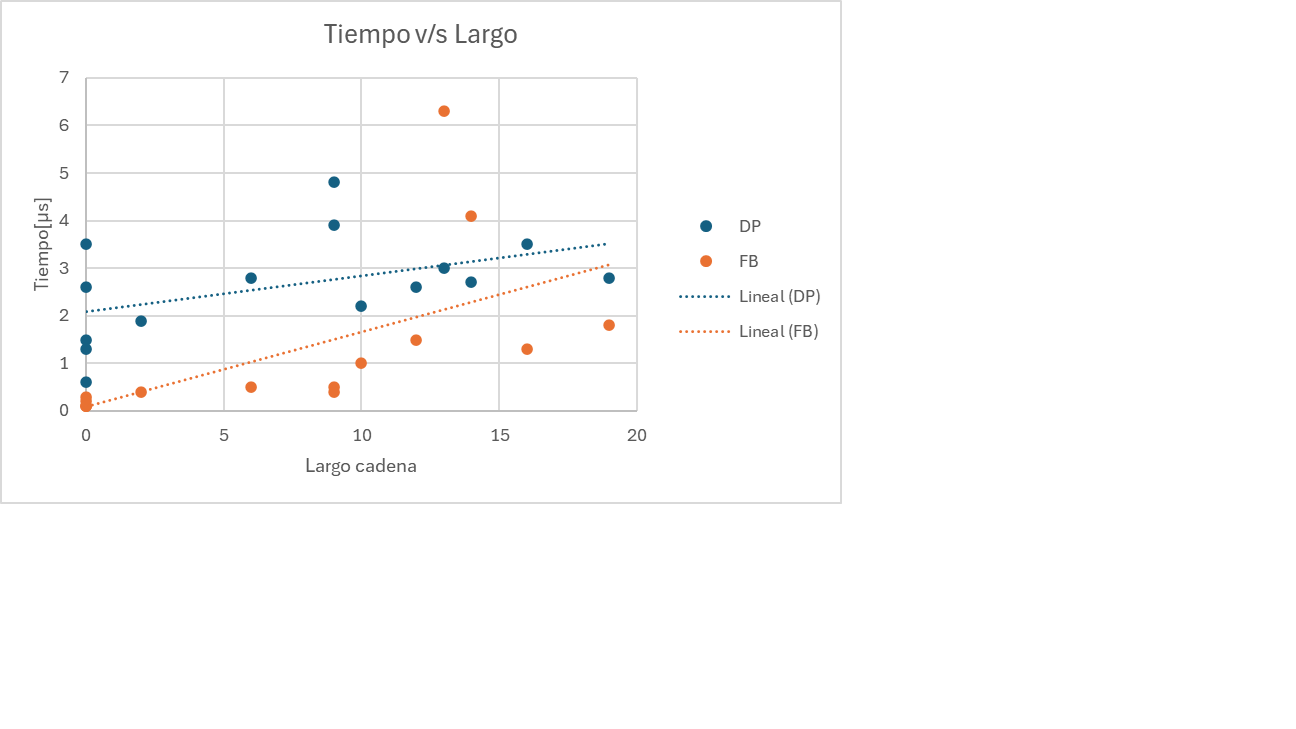
\includegraphics[width=\textwidth]{tikz/Grafico1.png}
        \caption{Gráfico correspondiente a Dataset1. Cadenas vacías.}
        \label{fig:dataset1}
    \end{figure}

    \item \textbf{Dataset2}: 
    \begin{figure}[H]
        \centering
        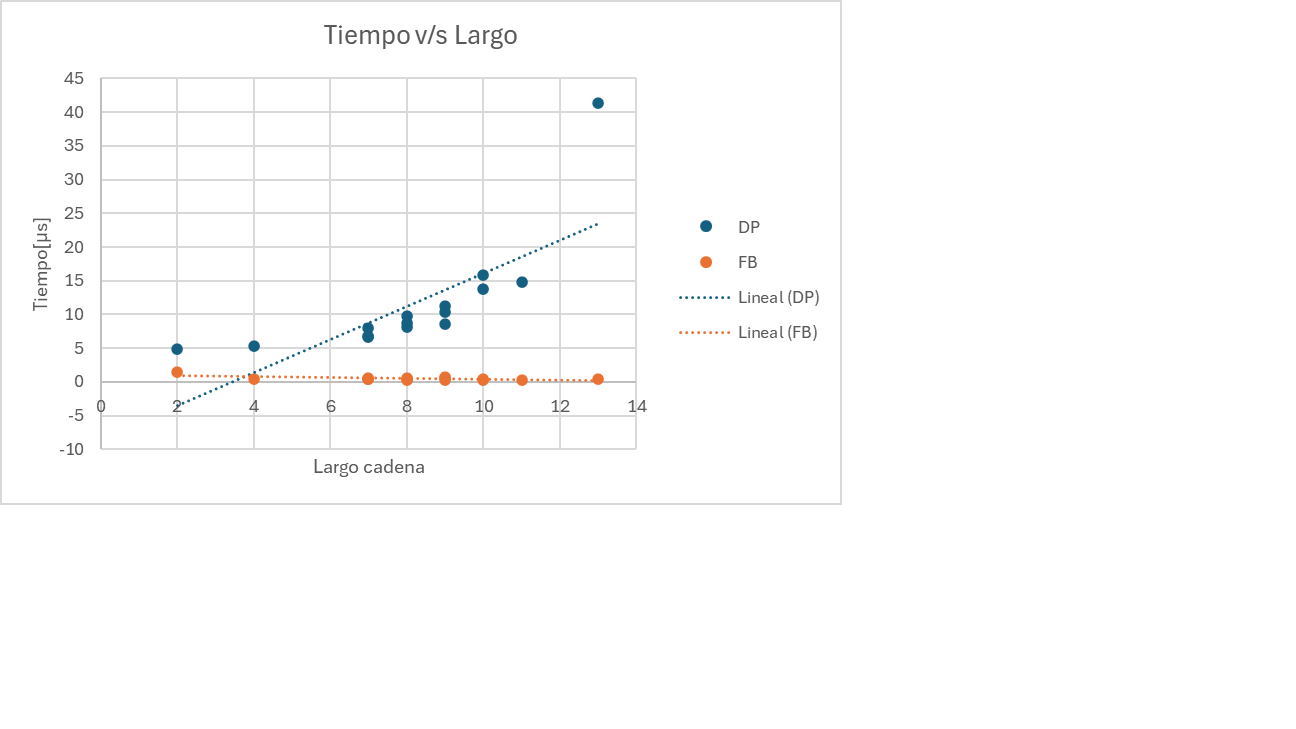
\includegraphics[width=\textwidth]{tikz/Grafico2.png}
        \caption{Gráfico correspondiente a Dataset2. Cadenas identicas.}
        \label{fig:dataset2}
    \end{figure}

    \item \textbf{Dataset3}: 
    \begin{figure}[H]
        \centering
        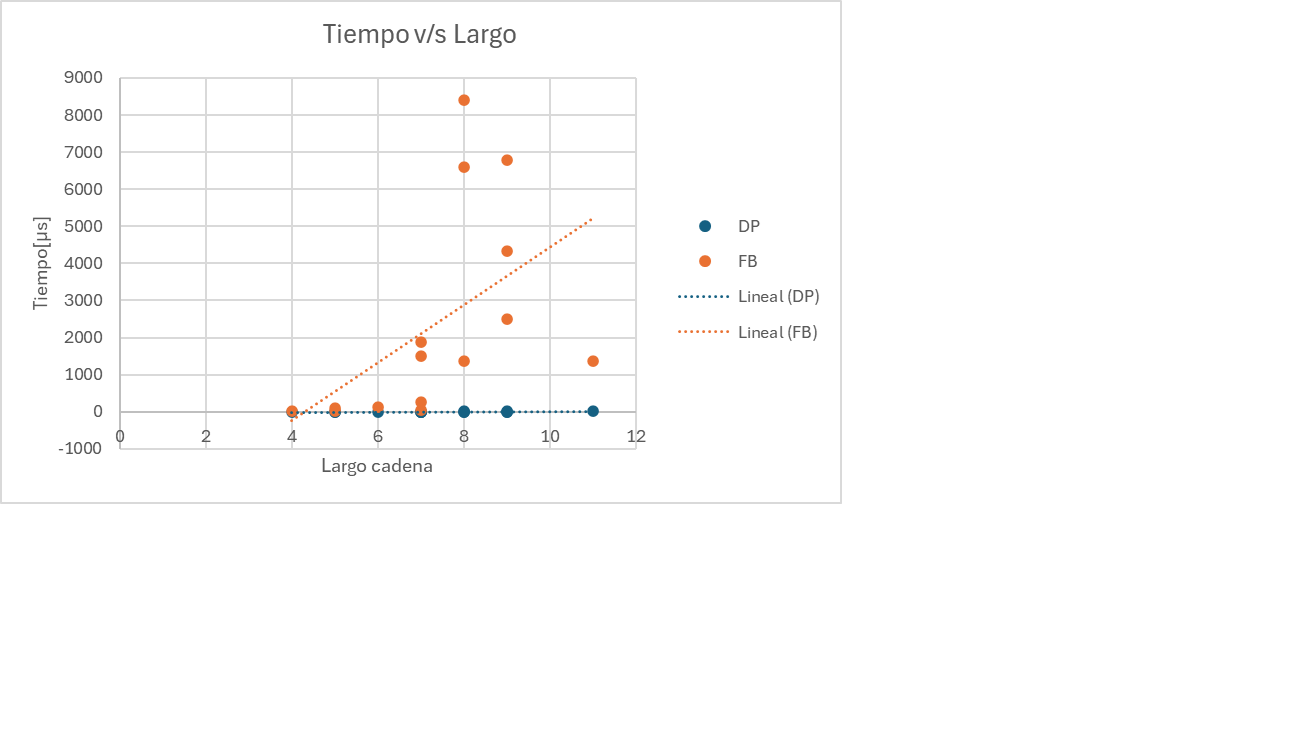
\includegraphics[width=\textwidth]{tikz/Grafico3.png}
        \caption{Gráfico correspondiente a Dataset3. Cadenas con caracteres repetidos.}
        \label{fig:dataset3}
    \end{figure}

    \item \textbf{Dataset4}: 
    \begin{figure}[H]
        \centering
        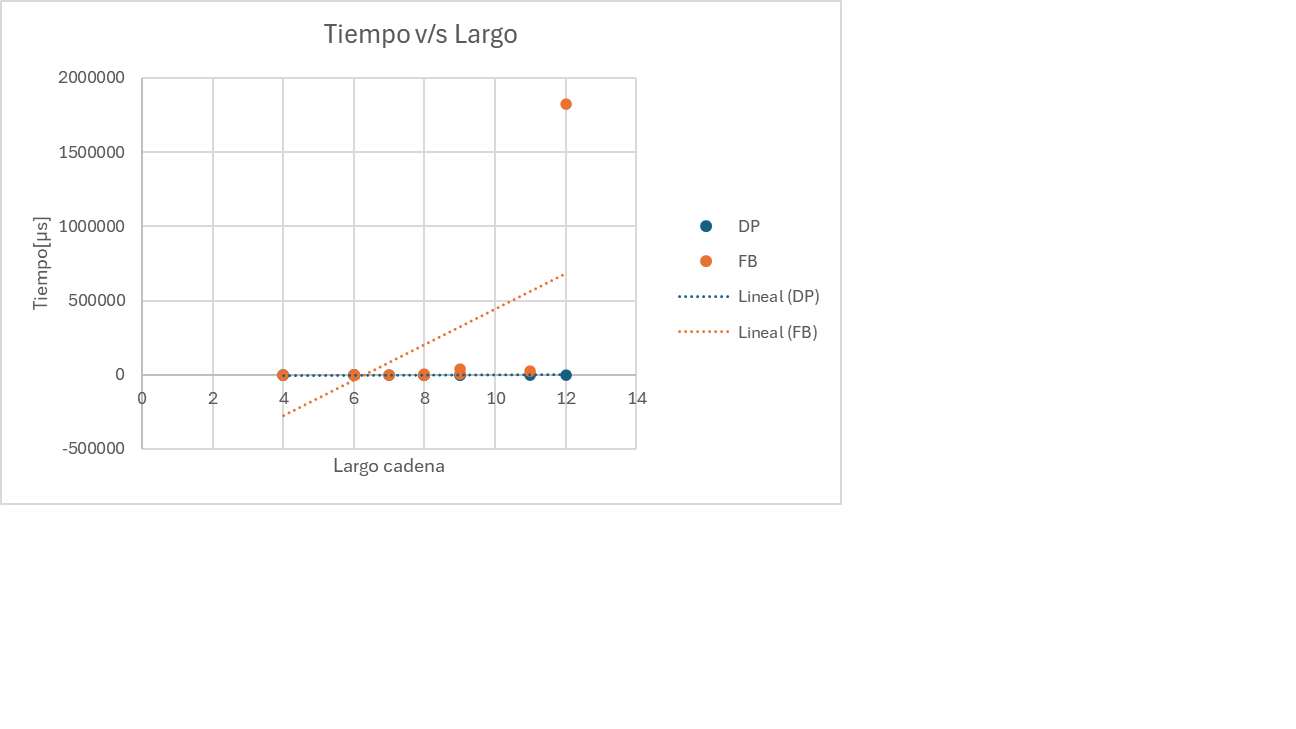
\includegraphics[width=\textwidth]{tikz/Grafico4.png}
        \caption{Gráfico correspondiente a Dataset4. Cadenas aleatorias con mismo tamaño.}
        \label{fig:dataset4}
    \end{figure}

    \item \textbf{Dataset5}: 
    \begin{figure}[H]
        \centering
        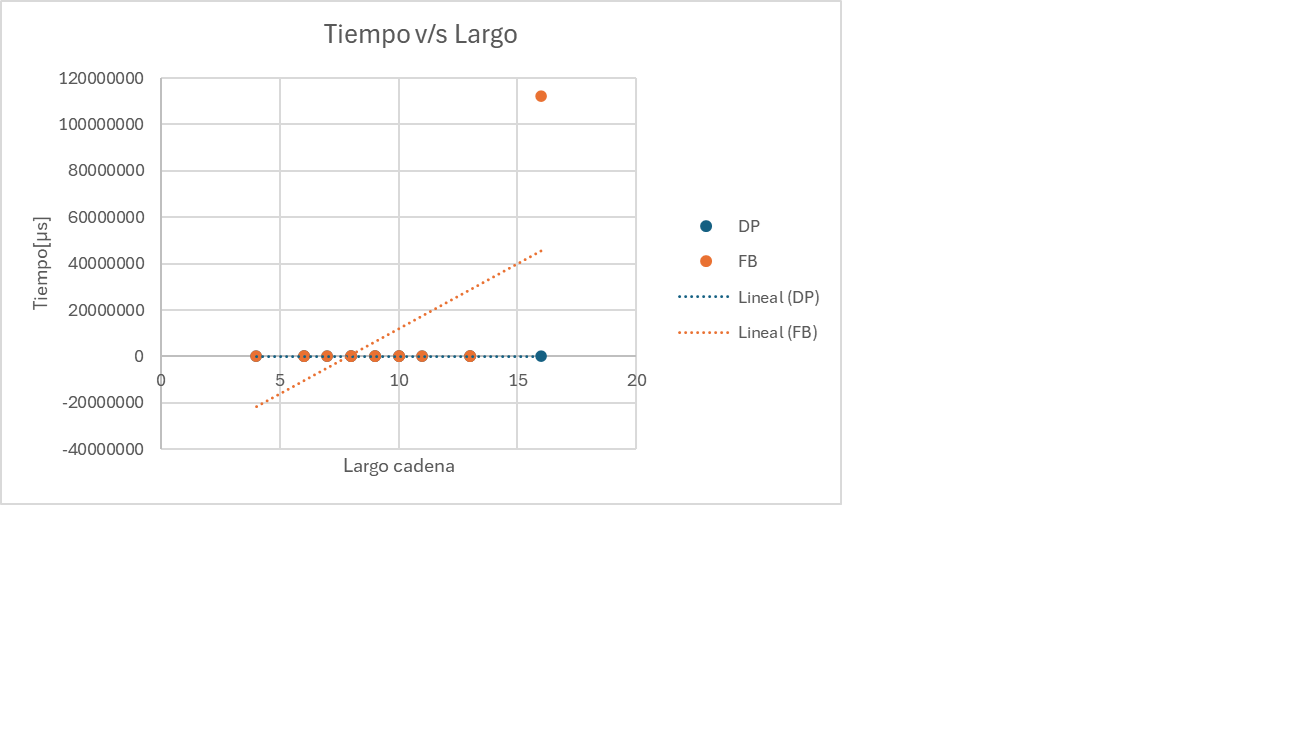
\includegraphics[width=\textwidth]{tikz/Grafico5.png}
        \caption{Gráfico correspondiente a Dataset5. Cadenas aleatorias con diferentes tamaños.}
        \label{fig:dataset5}
    \end{figure}

    \item \textbf{Dataset6}: 
    \begin{figure}[H]
        \centering
        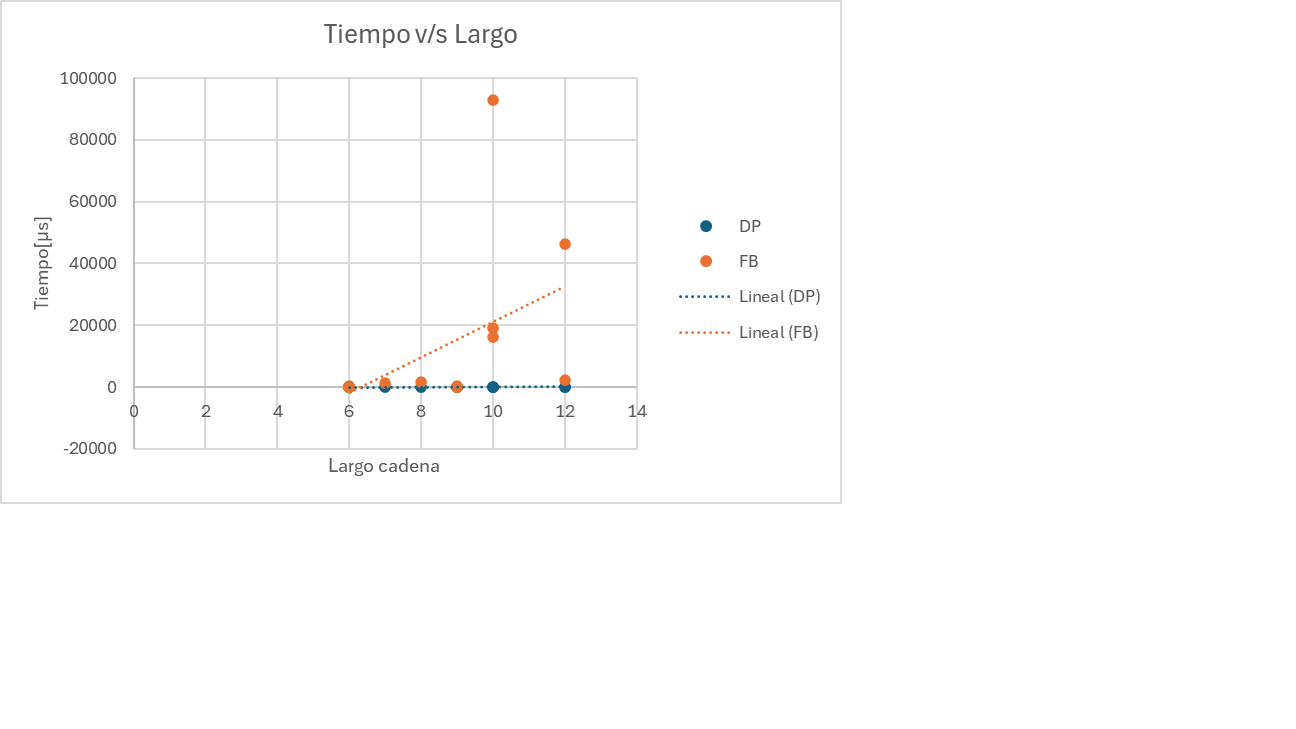
\includegraphics[width=\textwidth]{tikz/Grafico6.png}
        \caption{Gráfico correspondiente a Dataset6. cadenas con transposiciones.}
        \label{fig:dataset6}
    \end{figure}
\end{enumerate}


\newpage
\section{Conclusiones}
Basado en los resultados obtenidos, se observa que para cadenas vacías o cadenas totalmente idénticas, el algoritmo de fuerza bruta presenta tiempos de ejecución más bajos. Esto se debe a que, en estos casos, las recursiones terminan rápidamente al cumplirse siempre alguno de los casos base, lo que reduce significativamente el número de operaciones realizadas y genera un comportamiento cercano a constante. Por otro lado, el algoritmo de programación dinámica, independientemente de la entrada, debe recorrer y llenar completamente la matriz de soluciones parciales, lo que implica un mayor tiempo de ejecución en comparación con la fuerza bruta, incluso en casos simples.
En los casos en los que las cadenas no cumplen los casos base del algoritmo de fuerza bruta, se observa una tendencia notable en los tiempos de ejecución. A medida que aumenta el tamaño y la complejidad de las cadenas de entrada, el tiempo de ejecución del algoritmo de fuerza bruta crece exponencialmente, debido a la naturaleza combinatoria de las llamadas recursivas necesarias para evaluar todas las posibles soluciones. Este comportamiento es consistente con la complejidad temporal teórica previamente calculada para este algoritmo, lo que lo hace impráctico para entradas de tamaño considerable.

Por el contrario, el paradigma de programación dinámica muestra un crecimiento en los tiempos de ejecución mucho más controlado, siguiendo una tendencia lineal respecto al número de subproblemas resueltos. Este crecimiento más lento se alinea con la complejidad temporal cuadrática esperada, derivada de la construcción y evaluación de la matriz de soluciones parciales. Esto confirma la superioridad del enfoque de programación dinámica en términos de escalabilidad y eficiencia computacional cuando se trata de entradas grandes o complejas.

\newpage

\section{Condiciones de entrega}
% Condiciones generales de tareas de Algoritmos y Complejidad, 20231
  \begin{itemize}
  \item
    La tarea se realizará \tca{individualmente}
    (esto es grupos de una persona),
    sin excepciones.
  \item
    La entrega debe realizarse vía \url{http://aula.usm.cl}
    en un \tca{tarball} en el área designada al efecto,
    en el formato \tca{\texttt{tarea-\tnum-{rol}.tar.gz}}
    (\texttt{rol} con dígito verificador y sin guión).

    Dicho \tca{tarball} debe contener las fuentes en \LaTeXe{}
    (al menos \tca{\texttt{tarea-\tnum.tex}})
    de la parte escrita de su entrega,
    además de un archivo \tca{\texttt{tarea-\tnum.pdf}},
    correspondiente a la compilación de esas fuentes.
  \item Si se utiliza algún código, idea, o contenido extraído de otra fuente, este \textbf{debe} ser citado en el lugar exacto donde se utilice, en lugar de mencionarlo al final del informe. 
  \item
    Asegúrese que todas sus entregas tengan sus datos completos:
    número de la tarea, ramo, semestre, nombre y rol.
    Puede incluirlas como comentarios en sus fuentes \LaTeX{}
    (en \TeX{} comentarios son desde \% hasta el final de la línea)
    o en posibles programas.
    Anótese como autor de los textos.
 
  \item
    Si usa material adicional al discutido en clases,
    detállelo.
    Agregue información suficiente para ubicar ese material
    (en caso de no tratarse de discusiones con compañeros de curso
     u otras personas).
  \item No modifique \texttt{preamble.tex}, \texttt{tarea\_main.tex}, \texttt{condiciones.tex}, estructura de directorios, nombres de archivos, configuración del documento, etc. Sólo agregue texto, imágenes, tablas, código, etc. En el códigos funte de su informe, no agregue paquetes, ni archivos .tex (a excepción de que agregue archivos en \texttt{/tikz}, donde puede agregar archivos .tex con las fuentes de gráficos en \texttt{TikZ}).

\ifprograms
  \item
    Su programa ejecutable debe llamarse \tca{\texttt{tarea\tnum}},
    de haber varias preguntas solicitando programas,
    estos deben llamarse usando el número de la pregunta,
    como \tca{\texttt{tarea\tnum-1}},
    \tca{\texttt{tarea\tnum-2}},
    etc.
    Si hay programas compilados, con en este caso,
    incluya una \tca{\texttt{Makefile}}
    que efectúe las compilaciones correspondientes.

    Los programas se evalúan según que tan claros
    (bien escritos)
    son, si se compilan y ejecutan sin errores o advertencias según corresponda.
    Parte del puntaje es por ejecución correcta con casos de prueba.
    Si el programa no se ciñe a los requerimientos de entrada y salida,
    la nota respectiva es cero.
\fi    
  \item
    %La entrega debe realizarse dentro del plazo indicado en \url{http://aula.usm.cl}:
    La fecha límite de entrega es el día \tca{10 de noviembre de 2024}.

    \begin{center}
        \Large{
          \textbf{NO SE ACEPTARÁN TAREAS FUERA DE PLAZO}.
        }
        \normalsize
    \end{center}
     
    
  \item
    Nos reservamos el derecho de llamar a interrogación
    sobre algunas de las tareas entregadas.
    En tal caso,
    la nota de la tarea será la obtenida en la interrogación.
    \begin{center}
      \Large{
        \textbf{NO PRESENTARSE A UN LLAMADO A INTERROGACIÓN SIN JUSTIFICACIÓN PREVIA SIGNIFICA AUTOMÁTICAMENTE NOTA 0.}
      }
    \end{center}
    
  \end{itemize}

%%% Local Variables:
%%% mode: latex
%%% ispell-local-dictionary: "spanish"
%%% End:

  
% LocalWords:  tarball tar gz pdf min entregable Makefile puntaje
% LocalWords:  Moodle

\newpage
\appendix


\section{Apéndice 1}
Aquí puede agregar tablas, figuras u otro material que no se incluyó en el cuerpo principal del documento, ya que no constituyen elementos centrales de la tarea. Si desea agregar material adicional que apoye o complemente el análisis realizado, puede hacerlo en esta sección.

\begin{mdframed} 
    Esta sección es solo para material adicional. El contenido aquí no será evaluado directamente, pero puede ser útil si incluye material que será referenciado en el cuerpo del documento. Por lo tanto, asegúrese de que cualquier elemento incluido esté correctamente referenciado y justificado en el informe principal.
 \end{mdframed}


 
\printbibliography

\end{document}


